\section{Fundamentals of Estimation}
%This section is under Jazz-\work\\{\scriptsize [and will evolve from face-to-face interactions with students of mathematics at Uppsala University]}.

\subsection{Introduction}
Now that we have been introduced to two notions of convergence for RV sequences, we can begin to appreciate the basic limit theorems used in statistical inference.  The problem of estimation is of fundamental importance in statistical inference and learning.  We will formalise the general estimation problem here.  There are two basic types of estimation.  In point estimation we are interested in estimating a particular point of interest that is supposed to belong to a set of points.  In (confidence) set estimation, we are interested in estimating a set with a particular form that has a specified probability of ``trapping'' the particular point of interest from a set of points.  Here, a point should be interpreted as an element of a collection of elements from some space.

\subsection{Point Estimation}\label{S:PointEstimation}
{\bf Point estimation} is any statistical methodology that provides one with a ``{\bf single best guess}'' of some specific quantity of interest.  Traditionally, we denote this {\bf quantity of interest as $\theta^*$} and {\bf its point estimate as $\widehat{\theta}$ or $\widehat{\theta}_n$}.  The subscript $n$ in the point estimate $\widehat{\theta}_n$ emphasises that our estimate is based on $n$ observations or data points from a given statistical experiment to estimate $\theta^*$.  This quantity of interest, which is usually unknown, can be: %, namely $\theta$
%, may be an {\bf integral} $\Iz$ of a real valued function $h(x)$, i.e.~$\theta=\Iz := \int_a^b h(x)\,dx \in \Rz$, or simply a 
\begin{itemize}
\item an {\bf integral} $\vartheta^* := \int_A h(x)\,dx \in \BB{\varTheta}$.  If $\vartheta^*$ is finite, then $\BB{\varTheta} =  \Rz$, or %  For e.g.~see \ref{S:BMC} on Monte Carlo integration.
\item a {\bf parameter} $\theta^*$ which is an element of the {\bf parameter space} $\BB{\Theta}$, denoted $\theta^* \in \BB{\Theta}$,
\item a {\bf distribution function (DF)} $F^* \in \Fz := \text{the set of all DFs}$
\item a {\bf density function (pdf)} $f \in \{ \text{``not too wiggly Sobolev functions''} \}$, or 
\item a {\bf regression function} $g^* \in \Gz$, where $\Gz$ is a class of regression functions in a regression experiment with model: $Y=g^*(X)+\epsilon$, such that $\E(\epsilon)=0$, from pairs of observations $\{(X_i,Y_i)\}_{i=1}^n$, or
\item a {\bf classifier} $g^* \in \Gz$, i.e.~a regression experiment with discrete $Y = g^*(X)+\epsilon$, or 
\item a {\bf prediction} in a regression experiment, i.e.~when you want to estimate $Y_i$ given $X_i$. 
\end{itemize}
%\begin{table}[htpb]
%\begin{center}
%\begin{tabular}{|c c c|}
%\hline
%Quantity of Interest $\theta$ & Point Estimation & Sections \\ \hline
%Parameter $\theta \in \BB{\Theta} \subset \Rz^n$ & Parametric Estimation & Section~\ref*{S:ParametricEstimation} \\
%Integral $\Iz := \int_a^bh(x)\,dx$ & Monte Carlo Integration & Section~\ref*{S:BMC} \\ \hline
%\end{tabular}
%\end{center}
%\end{table}

Recall that a statistic is an RV $T(X)$ that maps every data point $x$ in the data space $\Xz$ with $T(x)=t$ in its range $\Tz$, i.e.~$T(x):\Xz \to \Tz$ (\hyperref[D:Statistic]{Definition~\ref*{D:Statistic}}).  Next, we look at a specific class of statistics whose range is the parameter space $\BB{\Theta}$.
\begin{definition}[Point Estimator]\label{D:Estimator}
A {\bf point estimator} $\widehat{\Theta}$ of some {\bf fixed and possibly unknown} $\theta^* \in \BB{\Theta}$ is a statistic that associates each data point $x \in \Xz$ with an estimate $\widehat{\Theta}(x)=\widehat{\theta} \in \BB{\Theta}$,  
\[
\boxed{
 \widehat{\Theta} := \widehat{\Theta}(x)=\widehat{\theta}: \Xz \to \BB{\Theta}
 } \ .
\]
If our data point $x := (x_1,x_2,\ldots,x_n)$ is an $n$-vector or a point in the $n$-dimensional real space, i.e.~$x := (x_1,x_2,\ldots,x_n) \in \Xz_n \subset \Rz^n$, then we emphasise the dimension $n$ in our point estimator $\widehat{\Theta}_n$ of $\theta^* \in \BB{\Theta}$.
\[
\boxed{
\widehat{\Theta}_n :=  \widehat{\Theta}_n(x:=(x_1,x_2,\ldots,x_n))=\widehat{\theta}_n : \Xz_n \to \BB{\Theta}, \quad \Xz_n \subset \Rz^n 
} \ .
\]
 The typical situation for us involves point estimation of $\theta^* \in \BB{\Theta}$ on the basis of one realisation $x \in\Xz_n \subset \Rz^n$ of an independent and identically distributed (IID) random vector $X=(X_1,X_2,\ldots,X_n)$, such that $X_1,X_2,\ldots,X_n \overset{\IID}{\sim} X_1$ and the DF of $X_1$ is $F(x_1; \theta^*)$, i.e.~the distribution of the IID RVs, $X_1, X_2,\ldots,X_n$, is parameterised by $\theta^* \in \BB{\Theta}$.
\end{definition}

\begin{example}[Coin Tossing Experiment ($X_1,\ldots,X_n \overset{IID}{\sim} \bernoulli(\theta^*)$)]\label{EX:CoinTossing}
I tossed a coin that has an unknown probability $\theta^*$ of landing Heads independently and identically $10$ times in a row.  Four of my outcomes were Heads and the remaining six were Tails, with the actual sequence of Bernoulli outcomes (Heads $\to 1$ and Tails $\to 0$) being $(1,0,0,0,1,1,0,0,1,0)$.  I would like to estimate the probability $\theta^* \in \BB{\Theta} = [0,1]$ of observing Heads using the natural estimator $\widehat{\Theta}_n((X_1,X_2,\ldots,X_n))$ of $\theta^*$:
\[
\widehat{\Theta}_n((X_1,X_2,\ldots,X_n)) := \widehat{\Theta}_n = \frac{1}{n} \sum_{i=1}^n X_i =: \overline{X}_n
\]
For the coin tossing experiment I just performed ($n=10$ times), the point estimate of the unknown $\theta^*$ is:
\begin{eqnarray}
\widehat{\theta}_{10} = \widehat{\Theta}_{10}((x_1,x_2,\ldots,x_{10})) 
&=&\widehat{\Theta}_{10}((1,0,0,0,1,1,0,0,1,0)) \notag \\
&=& \frac{1+0+0+0+1+1+0+0+1+0}{10}=\frac{4}{10}=0.40 \notag \ .
\end{eqnarray}
\end{example}

\begin{labwork}[$\bernoulli(38/75)$ Computer Experiment]\label{LW:1000CoinTossingExp}
Simulate one thousand IID samples from a $\bernoulli(\theta^*=38/75)$ RV and store this data in an array called $\tt Samples$.  Use your student ID to initialise the fundamental sampler.  Now, pretend that you don't know the true $\theta^*$ and estimate $\theta^*$ using our estimator $\widehat{\Theta}_n=\overline{X}_n$ from the data array $\tt Samples$ for each sample size $n=1,2,\ldots,1000$.  Plot the one thousand estimates $\widehat{\theta}_1,\widehat{\theta}_2,\ldots,\widehat{\theta}_{1000}$ as a function of the corresponding sample size.  Report your observations regarding the behaviour of our estimator as the sample size increases.
\end{labwork}

\subsection{Some Properties of Point Estimators}\label{S:PropPointEstim}
Given that an estimator is merely a function from the data space to the parameter space, we need choose only the best estimators available.  Recall that a point estimator $\widehat{\Theta}_n$, being a statistic or an RV of the data has a probability distribution over its range $\BB{\Theta}$.  This distribution over $\BB{\Theta}$ is called the {\bf sampling distribution} of $\widehat{\Theta}_n$.  Note that the sampling distribution not only depends on the statistic $\widehat{\Theta}_n := \widehat{\Theta}_n(X_1,X_2,\ldots,X_n)$ but also on $\theta^*$ which in turn determines the distribution of the IID data vector $(X_1,X_2,\ldots,X_n)$.  The following definitions are useful for selecting better estimators from some lot of them.

\begin{definition}[Bias of a Point Estimator]\label{D:Bias}
The $\mathsf{bias}_n$ of an estimator $\widehat{\Theta}_n$ of  $\theta^* \in \BB{\Theta}$ is:
\begin{equation}\label{E:Bias}
\boxed{
\mathsf{bias}_n=\mathsf{bias}_n(\widehat{\Theta}_n) := \E_{\theta^*}(\widehat{\Theta}_n) - \theta^* = \int_{\Xz_n} \widehat{\Theta}_n(x) \, dF(x;\theta^*) - \theta^*
}
 \ .
\end{equation} 
We say that the estimator $\widehat{\Theta}_n$ is {\bf unbiased} if $\mathsf{bias}_n(\widehat{\Theta}_n)=0$ or if $\E_{\theta^*}(\widehat{\Theta}_n)=\theta^*$ for every $n$.  If $\lim_{n \to \infty}\mathsf{bias}_n(\widehat{\Theta}_n)=0$, we say that the estimator is {\bf asymptotically unbiased}.
\end{definition}
Since the expectation of the sampling distribution of the point estimator $\widehat{\Theta}_n$ depends on the unknown $\theta^*$, we emphasise the $\theta^*$-dependence by $\E_{\theta^*}(\widehat{\Theta}_n)$.

\begin{example}[Bias of our Estimator of $\theta^*$]\label{EX:BiasEstimatePFromNIIDBernoulliTrials}
Consider the sample mean estimator $\widehat{\Theta}_n := \overline{X}_n$ of $\theta^*$, from $X_1,X_2,\ldots,X_n \overset{\IID}{\sim} \bernoulli(\theta^*)$.  That is, we take the sample mean of the $n$ IID $\bernoulli(\theta^*)$ trials to be our point estimator of $\theta^*\in[0,1]$.  Then, {\bf this estimator is unbiased} since:
\[
\E_{\theta^*}(\widehat{\Theta}_n) = \E_{\theta^*} \left( n^{-1} \sum_{i=1}^n X_i \right) = n^{-1} \E_{\theta^*} \left(  \sum_{i=1}^n X_i \right) = n^{-1} \sum_{i=1}^n \E_{\theta^*}(X_i) = n^{-1} n \theta^* = \theta^* \ .
\]
\end{example}

\begin{definition}[Standard Error of a Point Estimator]
The standard deviation of the point estimator $\widehat{\Theta}_n$ of  $\theta^* \in \BB{\Theta}$ is called the {\bf standard error}:
\begin{equation}\label{E:se}
\boxed{
\mathsf{se}_n = \mathsf{se}_n(\widehat{\Theta}_n)=\sqrt{\V_{\theta^*}(\widehat{\Theta}_n)} = \sqrt{ \int_{\Xz_n} \left( \widehat{\Theta}_n(x) - \E_{\theta^*}(\widehat{\Theta}_n) \right)^2 \, dF(x;\theta^*)}
}\ .
\end{equation}
\end{definition}
Since the variance of the sampling distribution of the point estimator $\widehat{\Theta}_n$ depends on the fixed and possibly unknown $\theta^*$, as emphasised by $\V_{\theta^*}$ in \eqref{E:se}, the $\mathsf{se}_n$ is also a possibly unknown quantity and may itself be estimated from the data.  The estimated standard error, denoted by $\widehat{\mathsf{se}}_n$, is calculated by replacing $\V_{\theta^*}(\widehat{\Theta}_n)$ in \eqref{E:se} with its appropriate estimate.

\begin{example}[Standard Error of our Estimator of $\theta^*$]\label{EX:StdErrEstimatePFromNIIDBernoulliTrials}
Consider the sample mean estimator $\widehat{\Theta}_n := \overline{X}_n$ of $\theta^*$, from $X_1,X_2,\ldots,X_n \overset{\IID}{\sim} \bernoulli(\theta^*)$.  Observe that the statistic: 
$$T_n((X_1,X_2,\ldots,X_n)) := n \,  \widehat{\Theta}_n((X_1,X_2,\ldots,X_n)) = \sum_{i=1}^n X_i$$ is the $\binomial(n,\theta^*)$ RV.
The standard error  $\mathsf{se}_n$ of this estimator is:
\[
\mathsf{se}_n=\sqrt{\V_{\theta^*}(\widehat{\Theta}_n)}
= \sqrt{\V_{\theta^*}\left(\sum_{i=1}^n \frac{X_i}{n} \right)}
= \sqrt{\left(\sum_{i=1}^n \frac{1}{n^2}\V_{\theta^*}(X_i) \right)}
= \sqrt{\frac{n}{n^2}\V_{\theta^*}(X_i)}
=\sqrt{{\theta^*}(1-{\theta^*})/n} \ .
\]
\end{example}

Another reasonable property of an estimator is that it converge to the ``true'' parameter $\theta^*$ -- here ``true'' means the supposedly fixed and possibly unknown $\theta^*$, as we gather more and more IID data from a $\theta^*$-specified DF $F(x; \theta^*)$.  This property is stated precisely next.
\begin{definition}[Asymptotic Consistency of a Point Estimator]\label{D:Consistency}
A point estimator $\widehat{\Theta}_n$ of $\theta^* \in \BB{\Theta}$ is said to be {\bf asymptotically consistent} if:
\[
\boxed{
\widehat{\Theta}_n \overset{P}{\longrightarrow} \theta^*
} \qquad \text{i.e., for any real $\epsilon > 0$,} \quad
\boxed{
\lim_{n \to \infty} \P (| \widehat{\Theta}_n - \theta^* | > \epsilon) = 0
} \ .
\]
\end{definition}

\begin{definition}[Mean Squared Error (MSE) of a Point Estimator]\label{D:MSE}
Often, the quality of a point estimator $\widehat{\Theta}_n$ of $\theta^* \in \BB{\Theta}$ is assessed by the {\bf mean squared error} or $\mathsf{MSE}_n$ defined by:
\begin{equation}\label{E:MSE}
\boxed{
\mathsf{MSE}_n=\mathsf{MSE}_n(\widehat{\Theta}_n) := \E_{\theta^*} \left((\widehat{\Theta}_n-\theta^*)^2 \right) 
= \int_{\Xz} (\widehat{\Theta}_n(x)-\theta^*)^2 \, dF(x;\theta^*) 
} \ .
\end{equation}
\end{definition}

The following proposition shows a simple relationship between the mean square error, bias and variance of an estimator $\widehat{\Theta}_n$ of $\theta^*$.
\begin{prop}[The $\sqrt{\mathsf{MSE}_n}:\mathsf{se}_n:\mathsf{bias}_n$--Sided Right Triangle of an Estimator]
Let $\widehat{\Theta}_n$ be an estimator of $\theta^* \in \BB{\Theta}$.  Then:
\begin{equation}\label{E:RMseSeBiasTriangle}
\boxed{
\mathsf{MSE}_n(\widehat{\Theta}_n) 
= (\mathsf{se}_n(\widehat{\Theta}_n))^2 + (\mathsf{bias}_n(\widehat{\Theta}_n))^2
} \ .
\end{equation}
{\scriptsize
\begin{proof}
\begin{eqnarray}
& & LHS \notag \\
&=& \mathsf{MSE}_n(\widehat{\Theta}_n) \notag \\
&:=& \E_{\theta^*} \left((\widehat{\Theta}_n-\theta^*)^2 \right), \qquad  \text{by definition of $\mathsf{MSE}_n$ \eqref{E:MSE}} \notag \\
&=& \E_{\theta^*} \left( \left( \ \underset{A}{\underbrace{\left(\widehat{\Theta}_n -\E_{\theta^*}(\widehat{\Theta}_n) \right)}} + \underset{B}{\underbrace{\left(\E_{\theta^*}(\widehat{\Theta}_n) -\theta^* \right)}} \ \right)^2 \right), \qquad \text{by subtracting and adding the constant $\E_{\theta^*}(\widehat{\Theta}_n)$} \notag \\
&=& \E_{\theta^*} \left( \underset{A^2}{\underbrace{{\left(\widehat{\Theta}_n -\E_{\theta^*}(\widehat{\Theta}_n) \right)}^2}} + \underset{2AB}{\underbrace{2  {\left(\widehat{\Theta}_n -\E_{\theta^*}(\widehat{\Theta}_n) \right)} {\left(\E_{\theta^*}(\widehat{\Theta}_n) -\theta^* \right)}}} + \underset{B^2}{\underbrace{{\left(\E_{\theta^*}(\widehat{\Theta}_n) -\theta^* \right)}^2}}  \right), \qquad \text{$\because \ (A+B)^2=A^2+2AB+B^2$} \notag \\
&=& \E_{\theta^*} \left( {\left(\widehat{\Theta}_n -\E_{\theta^*}(\widehat{\Theta}_n) \right)}^2 \right) + 
\E_{\theta^*} \left( 2  {\left(\widehat{\Theta}_n -\E_{\theta^*}(\widehat{\Theta}_n) \right)} {\left(\E_{\theta^*}(\widehat{\Theta}_n) -\theta^* \right)} \right) + 
\E_{\theta^*} \left( {\left(\E_{\theta^*}(\widehat{\Theta}_n) -\theta^* \right)}^2  \right), %\quad \text{taking $\E_{\theta^*}(\cdot)$ of $A^2$, $2AB$ and $B^2$} 
\notag \\
&=& \E_{\theta^*} \left( {\left(\widehat{\Theta}_n -\E_{\theta^*}(\widehat{\Theta}_n) \right)}^2 \right) + 
\underset{C}{\underbrace{2 {\left(\E_{\theta^*}(\widehat{\Theta}_n) -\theta^* \right)}}} \underset{D}{\underbrace{ \E_{\theta^*} \left(  {\left(\widehat{\Theta}_n -\E_{\theta^*}(\widehat{\Theta}_n) \right)} \right)}} + 
\E_{\theta^*} \left( {\left(\E_{\theta^*}(\widehat{\Theta}_n) -\theta^* \right)}^2  \right), \quad \text{$\because \ C$ 
% := 2 {\left(\E_{\theta^*}(\widehat{\Theta}_n) -\theta^* \right)}$
is constant} \notag \\
&=& \E_{\theta^*} \left( {\left(\widehat{\Theta}_n -\E_{\theta^*}(\widehat{\Theta}_n) \right)}^2 \right) + 
0 + 
\E_{\theta^*} \left( {\left(\E_{\theta^*}(\widehat{\Theta}_n) -\theta^* \right)}^2  \right), \qquad \text{$\because \ D := \E_{\theta^*} \left(  {\left(\widehat{\Theta}_n -\E_{\theta^*}(\widehat{\Theta}_n) \right)} \right)=\E_{\theta^*}(\widehat{\Theta}_n ) - \E_{\theta^*}(\widehat{\Theta}_n) = 0$} \notag \\
&=& \V_{\theta^*}(\widehat{\Theta}_n)+ 
\E_{\theta^*} \left( {\left(\E_{\theta^*}(\widehat{\Theta}_n) -\theta^* \right)}^2  \right), \qquad \text{$\because \ \V_{\theta^*}(\widehat{\Theta}_n) := \E_{\theta^*} \left( {\left(\widehat{\Theta}_n -\E_{\theta^*}(\widehat{\Theta}_n) \right)}^2 \right)$, by definition of variance} \notag \\
&=& \left( \sqrt{\V_{\theta^*}(\widehat{\Theta}_n)} \right)^2+ 
\E_{\theta^*} \left( {\left( \mathsf{bias}_n(\widehat{\Theta}_n) \right)}^2  \right), \qquad \text{$\because \  \mathsf{bias}_n(\widehat{\Theta}_n) = \E_{\theta^*}(\widehat{\Theta}_n) -\theta^* $, by definition of $\mathsf{bias}_n$ of an estimator $\widehat{\Theta}_n$} \notag \\
&=&  \left(  \mathsf{se}_n(\widehat{\Theta}_n) \right)^2 + 
\E_{\theta^*} \left( {\left( \mathsf{bias}_n(\widehat{\Theta}_n) \right)}^2  \right) , \qquad 
\text{$\because \ \mathsf{se}_n(\widehat{\Theta}_n) := \sqrt{\V_{\theta^*}(\widehat{\Theta}_n)}$, by definition \eqref{E:se}} \notag \\
&=&  \left(  \mathsf{se}_n(\widehat{\Theta}_n) \right)^2 + 
 {\left( \mathsf{bias}_n(\widehat{\Theta}_n) \right)}^2, \qquad 
\text{$\because \  \mathsf{bias}_n(\widehat{\Theta}_n) = \E_{\theta^*}(\widehat{\Theta}_n) -\theta^*$ and $\left( \mathsf{bias}_n(\widehat{\Theta}_n) \right)^2$ are constants.} \notag \\
&=& RHS \notag 
\end{eqnarray}
\end{proof}
}
\end{prop}

\begin{prop}[Asymptotic consistency of a point estimator]\label{P:AsympConsistencyUnbiasedSE0}
Let $\widehat{\Theta}_n$ be an estimator of $\theta^* \in \BB{\Theta}$.  Then, if $\mathsf{bias}_n(\widehat{\Theta}_n) \to 0$ and $\mathsf{se}_n(\widehat{\Theta}_n) \to 0$ as $n \to \infty$, the estimator $\widehat{\Theta}_n$ is asymptotically consistent:
\[
\widehat{\Theta}_n \overset{P}{\longrightarrow} \theta^* \ .
\]
{\scriptsize
\begin{proof}
If $\mathsf{bias}_n(\widehat{\Theta}_n) \to 0$ and $\mathsf{se}_n(\widehat{\Theta}_n) \to 0$, then by \eqref{E:RMseSeBiasTriangle}, $\mathsf{MSE}_n(\widehat{\Theta}_n) \to 0$, i.e.~that $\E_{\theta^*}\left( (\widehat{\Theta}_n-\theta^*)^2 \right) \to 0$.  This type of convergence of the RV $\widehat{\Theta}_n$ to the $Point~Mass(\theta^*)$ RV as $n \to \infty$ is called convergence in {\bf quadratic mean} or {\bf convergence in} $\B{L_2}$ and denoted by $\widehat{\Theta}_n \overset{qm}{\longrightarrow} \theta^*$.  Convergence in quadratic mean is a stronger notion of convergence than convergence in probability, in the sense that 
\[
\E_{\theta^*}\left( (\widehat{\Theta}_n-\theta^*)^2 \right) \to 0 \quad \text{ or } \quad \widehat{\Theta}_n \overset{qm}{\longrightarrow} \theta^* \implies \widehat{\Theta}_n \overset{P}{\longrightarrow} \theta^* \ .
\]
Thus, if we prove the above implication we are done with the proof of our proposition.  To show that convergence in quadratic mean implies convergence in probability for general sequence of RVs $X_n$ converging to an RV $X$, we first assume that $X_n \overset{qm}{\longrightarrow} X$.
Now, fix any $\epsilon>0$.  Then by Markov's inequality \eqref{E:MarkovNeq},
\[
\P(|X_n-X|>\epsilon) = \P(|X_n-X|^2>\epsilon^2) \leq \frac{\E(|X_n-X|^2)}{\epsilon^2} \to 0 \ ,
\]
and we have shown that the definition of convergence in probability holds provided convergence in quadratic mean holds.
\end{proof}
}
\end{prop}
We want our estimator to be unbiased with small standard errors as the sample size $n$ gets large.  The {\bf point estimator} $\widehat{\Theta}_n$ will then produce a {\bf point estimate} $\widehat{\theta}_n$:
$$\widehat{\Theta}_n((x_1,x_2,\ldots,x_n)) = \widehat{\theta}_n \in \BB{\Theta} \enspace ,$$ on the basis of the {\bf observed data} $(x_1,x_2,\ldots,x_n)$, that is close to the {\bf true parameter} $\theta^* \in \BB{\Theta}$.

\begin{example}[Asymptotic consistency of our Estimator of $\theta^*$]
Consider the sample mean estimator $\widehat{\Theta}_n := \overline{X}_n$ of $\theta^*$, from $X_1,X_2,\ldots,X_n \overset{\IID}{\sim} \bernoulli(\theta^*)$.  Since $\mathsf{bias}_n(\widehat{\Theta}_n)=0$ for any $n$ and 
$\mathsf{se}_n=\sqrt{\theta^*(1-\theta^*)/n} \to 0$, as $n \to \infty$, by 
\hyperref[P:AsympConsistencyUnbiasedSE0]{Proposition \ref*{P:AsympConsistencyUnbiasedSE0}}, 
$\widehat{\Theta}_n \overset{P}{\longrightarrow} \theta^*$.  That is $\widehat{\Theta}_n$ is an {\bf asymptotically consistent estimator} of $\theta^*$.  
\end{example}

\subsection{Confidence Set Estimation}\label{S:ConfidenceSets}
As we saw in Section~\ref*{S:PointEstimation}, the point estimate $\widehat{\theta}_n$ is a ``single best guess'' of  the fixed and possibly unknown parameter $\theta^* \in \BB{\Theta}$.  However, if we wanted to make a statement about our confidence in an estimation procedure, then one possibility is to produce subsets from the parameter space $\BB{\Theta}$ called {\bf confidence sets} that ``engulf'' $\theta^*$ with a probability of at least $1-\alpha$.  

Formally, an $1-\alpha$ {\bf confidence interval} for the parameter $\theta^* \in \BB{\Theta} \subset \Rz$, based on $n$ observations or data points $X_1,X_2,\ldots,X_n$, is an interval $C_n$ that is a function of the data:
\[
C_n := [\underline{C}_{\, n}, \overline{C}_{\, n}]
= [\underline{C}_{\, n}(X_1,X_2,\ldots,X_n), \overline{C}_{\, n}(X_1,X_2,\ldots,X_n)] \ ,
\]
such that:
\[
\P_{\theta^*} \left(  \theta^* \in C_n :=  [\underline{C}_{\, n}, \overline{C}_{\, n}] \right) \geq 1-\alpha \ .
\]
Note that the confidence interval $C_n := [\underline{C}_{\, n}, \overline{C}_{\, n}]$ is a two-dimensional RV or a random vector in $\Rz^2$ that depends on the two statistics $\underline{C}_{\, n} (X_1,X_2,\ldots,X_n) $ and $\overline{C}_{\, n} (X_1,X_2,\ldots,X_n) $, as well as $\theta^*$, which in turn determines the distribution of the data $(X_1,X_2,\ldots,X_n)$.  In words, $C_n$ engulfs the true parameter $\theta^* \in \BB{\Theta}$ with a probability of at least $1-\alpha$.  We call $1-\alpha$ as the {\bf coverage} of the confidence interval $C_n$.

Formally, a $1-\alpha$ {\bf confidence set} $C_n$ for a vector-valued $\theta^* \in \BB{\Theta} \subset \Rz^k$ is any subset of $\BB{\Theta}$ such that $\P_{\theta^*}( \theta^* \in C_n) \geq 1-\alpha$.  The typical forms taken by $C_n$ are $k$-dimensional boxes or hyper-cuboids, hyper-ellipsoids and subsets defined by inequalities involving level sets of some estimator of $\theta^*$.  

Typically, we take $\alpha=0.05$ because we are interested in the $1-\alpha=0.95$ or $95\%$ confidence interval/set $C_n \subset \BB{\Theta}$ of $\theta^* \in \BB{\Theta}$ from an estimator $\widehat{\Theta}_n$ of $\theta^*$.  

%Let us look at an example that makes use of the CLT next.
%\begin{example}[Errors in computer code (Wasserman03, p.~78)]\label{EX:CLTPoisson}
%Suppose the collection of RVs $X_1,X_2, \ldots, X_n$ model the number of errors in $n$ computer programs named $1,2,\ldots,n$, respectively.  Suppose that the RV $X_i$ modelling the number of errors in the $i^{\text{th}}$ program is the $Poisson(\lambda^*=5)$ for any $i=1,2,\ldots,n$.  Also suppose that they are independently distributed.  In short, we suppose that:
%\[
%X_1,X_2,\ldots,X_n \overset{\IID}{\sim} \poisson(\lambda^*=5) \ . 
%\]
%Suppose we have $n=125$ programs and want to make a probability statement about $\overline{X}_n$ which is the average number of errors per program out of these $125$ programs.  Since $\E(X_i) = \lambda^*=5$ and $\V(X_i)=\lambda^*=5$, we may want to know how often our sample mean $\overline{X}_{125}$ differs from the expectation of $5$ errors per program.  Using the CLT, we can approximate $\P(\overline{X}_n < 5.5)$, for instance, as follows:
%\begin{eqnarray}
%\P(\overline{X}_n < 5.5) 
%&=& \P \left( \frac{\sqrt{n}(\overline{X}_n - \E(X_1))}{\sqrt{\V(X_1)}} < \frac{\sqrt{n}(5.5-\E(X_1))}{\sqrt{\V(X_1)}} \right) \notag \\
%&\approxeq& \P \left( Z < \frac{\sqrt{n}(5.5-\lambda^*)}{\sqrt{\lambda^*}} \right) \qquad \text{{\scriptsize [by \eqref{E:CLTApprox}, and $\E(X_1)=\V(X_1)=\lambda^*$]}} \notag \\
%&=& \P \left( Z < \frac{\sqrt{125}(5.5-5)}{\sqrt{5}} \right) \qquad \text{{\scriptsize [Since, $\lambda^*=5$ and $n=125$ in this Example]}} \notag \\
%&=& \P(Z \leq 2.5) = \Phi(2.5) =  \int_{- \infty}^{2.5} \left( \frac{1}{\sqrt{2 \pi}} \ \exp \left( \frac{-x^2}{2} \right) \right) dx \approxeq 0.993790334674224 \ . \notag
%\end{eqnarray}
%To obtain the final number in this approximation, we need the following:
%\begin{labwork}
%The numerical approximation of $\Phi(2.5)$ was obtained via the call shown below to our $\erf$-based {\tt NormalCdf} function from \ref*{Mf: NormalCdfPdf}.  We could have also found it from a pre-computed Table for $\Phi(x)$.
%\begin{VrbM}
%>> format long
%>> disp(NormalCdf(2.5,0,1))
%   0.993790334674224
%\end{VrbM}
%\end{labwork}
%\end{example}

The CLT says that if $X_1,X_2,\ldots \overset{\IID}{\sim} X_1$ then $Z_n := \sqrt{n}(\overline{X}_n-\E(X_1))/\sqrt{\V(X_1)}$ is approximately distributed as $\normal(0,1)$.  In \hyperref[EX:CLTPoisson]{Example \ref*{EX:CLTPoisson}}, we knew $\sqrt{\V(X_1)}$ since we assumed knowledge of $\lambda^*=5$.   However, in general, we may not know $\sqrt{\V(X_1)}$.  The next proposition says that we may estimate $\sqrt{\V(X_1)}$ using the sample standard deviation $S_n$ of $X_1,X_2,\ldots,X_n$, according to \eqref{E:SampleStdDevRV}, and still make probability statements about the sample mean $\overline{X}_n$ using a $\normal$ distribution, {\bf provided $\mathbf{n}$ is not too small}, for e.g.~$n \geq 30$.
\begin{prop}[CLT based on Sample Variance]
Let $X_1,X_2,\ldots \overset{\IID}{\sim} X_1$ and suppose $\E(X_1)$ and $\V(X_1)$ exists, then:
\begin{equation}\label{E:CLTApproxSn}
\frac{\sqrt{n} \left( \overline{X}_n - \E(X_1) \right)}{S_n} \rightsquigarrow \normal(0,1) \ .
\end{equation}
\end{prop}

The following property of an estimator makes it easy to obtain confidence intervals.
\begin{definition}[Asymptotic Normality of Estimators]
An estimator $\widehat{\Theta}_n$ of a fixed and possibly unknown parameter $\theta^* \in \BB{\Theta}$ is {\bf asymptotically normal} if:
\begin{equation}\label{E:AsymptoticNormalEstimator}
\frac{\widehat{\Theta}_n - \theta^*}{\mathsf{se}_n} \rightsquigarrow \normal(0,1) \ .
\end{equation} 
That is, $\widehat{\Theta}_n \rightsquigarrow \normal(\theta^*,\mathsf{se}_n^2)$.  By a further estimation of $\mathsf{se}_n := \sqrt{\V_{\theta^*}(\widehat{\Theta}_n)}$ by $\widehat{\mathsf{se}}_n$, we can see that $\widehat{\Theta}_n \rightsquigarrow \normal(\theta^*,\widehat{\mathsf{se}}_n^2)$ on the basis of \eqref{E:CLTApproxSn}.
\end{definition}

\begin{prop}[Normal-based Asymptotic Confidence Interval]\label{P:NormalBasedAsympCI}
Suppose an estimator $\widehat{\Theta}_n$ of  parameter $\theta^* \in \BB{\Theta} \subset \Rz$ is asymptotically normal:
\[
\widehat{\Theta}_n \rightsquigarrow \normal(\theta^*,\widehat{\mathsf{se}}_n^2) \ .
\]
Let the RV $Z \sim \normal(0,1)$ have DF $\Phi$ and inverse DF $\Phi^{-1}$.  Let:
\[
z_{\alpha/2}=\Phi^{-1}(1-(\alpha/2)), \quad \text{ that is, } \quad \P(Z>z_{\alpha/2})=\alpha/2 \ \text{ and } \ \P(-z_{\alpha/2} < Z < z_{\alpha/2}) = 1-\alpha \ .
\]
Then:
\[
\P_{\theta^*}(\theta^* \in C_n)  = \P \left( \theta^* \in [\widehat{\Theta}_n - z_{\alpha/2} \widehat{\mathsf{se}}_n, \widehat{\Theta}_n + z_{\alpha/2} \widehat{\mathsf{se}}_n] \right) \to 1-\alpha \ .
\]
Therefore:
\[
C_n := [\underline{C}_{\, n}, \overline{C}_{\, n}]
= [\widehat{\Theta}_n - z_{\alpha/2} \widehat{\mathsf{se}}_n, \widehat{\Theta}_n + z_{\alpha/2} \widehat{\mathsf{se}}_n]
\] 
is the $1-\alpha$ Normal-based asymptotic confidence interval that relies on the asymptotic normality of the estimator $\widehat{\Theta}_n$ of $\theta^* \in \BB{\Theta} \subset \Rz$.
{\scriptsize
\begin{proof}
Define the centralised and scaled estimator as $Z_n := (\widehat{\Theta}_n-\theta^*)/\widehat{\mathsf{se}}_n$.  By assumption, $Z_n \rightsquigarrow Z \sim \normal(0,1)$.  Therefore,
\begin{eqnarray}
\P_{\theta^*}(\theta^* \in C_n) 
&=& \P_{\theta^*} \left( \theta^* \in [\widehat{\Theta}_n - z_{\alpha/2} \widehat{\mathsf{se}}_n, \widehat{\Theta}_n + z_{\alpha/2} \widehat{\mathsf{se}}_n] \right) \notag \\
&=& \P_{\theta^*} \left( \widehat{\Theta}_n - z_{\alpha/2} \widehat{\mathsf{se}}_n \leq \theta^* \leq  \widehat{\Theta}_n + z_{\alpha/2} \widehat{\mathsf{se}}_n \right) \notag \\
&=& \P_{\theta^*} \left(  - z_{\alpha/2} \widehat{\mathsf{se}}_n \leq \widehat{\Theta}_n - \theta^* \leq   z_{\alpha/2} \widehat{\mathsf{se}}_n \right) \notag \\
&=& \P_{\theta^*} \left(  - z_{\alpha/2}  \leq \frac{\widehat{\Theta}_n - \theta^*}{\widehat{\mathsf{se}}_n} \leq   z_{\alpha/2} \right) \notag \\
&\to& \P_{\theta^*} \left(  - z_{\alpha/2}  \leq Z \leq   z_{\alpha/2} \right) \notag \\
&=& 1-\alpha \notag
\end{eqnarray}
\end{proof}
}
\begin{figure}[htb]
\caption{Density and Confidence Interval of the Asymptotically Normal Point Estimator}
\vspace{4cm}
\end{figure}
For $95\%$ confidence intervals, $\alpha=0.05$ and $z_{\alpha/2}=z_{0.025}=1.96\approxeq 2$.  This leads to the {\bf approximate ${95\%}$ confidence interval} of $\widehat{\theta}_n \pm 2 \widehat{\mathsf{se}}_n$, where $\widehat{\theta}_n=\widehat{\Theta}_n(x_1,x_2,\ldots,x_n)$ and $x_1,x_2,\ldots,x_n$ are the data or observations of the RVs $X_1,X_2,\ldots,X_n$.
\end{prop}

\begin{example}[Confidence interval for $\theta^*$ from $n$ $\bernoulli(\theta^*)$ trials]\label{EX:EstimatePFromNIIDBernoulliTrials}
Let $X_1,X_2,\ldots,X_n \overset{\IID}{\sim} \bernoulli(\theta^*)$ for some fixed but unknown parameter $\theta^* \in \BB{\Theta}=[0,1]$.  Consider the following point estimator of $\theta^*$:
\[
\widehat{\Theta}_n((X_1,X_2,\ldots,X_n)) = n^{-1} \sum_{i=1}^n X_i \ .
\]
That is, we take the sample mean of the $n$ IID $\bernoulli(\theta^*)$ trials to be our point estimator of $\theta^*\in[0,1]$.  Then, we already saw that {\bf this estimator is unbiased}

We already saw that the standard error  $\mathsf{se}_n$ of this estimator is:
\[
\mathsf{se}_n=\sqrt{{\theta^*}(1-{\theta^*})/n} \ .
\]
Since ${\theta^*}$ is unknown, we obtain the estimated standard error $\widehat{\mathsf{se}}_n$ from the point estimate $\widehat{\theta}_n$ of ${\theta^*}$ on the basis of $n$ observed data points $x=(x_1,x_2,\ldots,x_n)$ of the experiment:
\[
\widehat{\mathsf{se}}_n = \sqrt{\widehat{\theta}_n(1-\widehat{\theta}_n)/n}, \quad \text{where, } \quad \widehat{\theta}_n=\widehat{\Theta}_n((x_1,x_2,\ldots,x_n))=n^{-1}\sum_{i=1}^n x_i \ .
\]
By the central limit theorem, $\widehat{\Theta}_n \rightsquigarrow \normal(\theta^*,\widehat{\mathsf{se}}_n)$, i.e.~$\widehat{\Theta}_n$ is asymptotically normal.  Therefore, an asymptotically (for large sample size $n$) approximate $1-\alpha$ normal-based confidence interval is:
\[
\widehat{\theta}_n \pm z_{\alpha/2} \widehat{\mathsf{se}}_n 
= \widehat{\theta}_n \pm z_{\alpha/2} \sqrt{\frac{ \widehat{\theta}_n (1- \widehat{\theta}_n )}{n}}
:= \left[ \, \widehat{\theta}_n - z_{\alpha/2} \sqrt{\frac{ \widehat{\theta}_n (1- \widehat{\theta}_n )}{n}} \ , \ \widehat{\theta}_n + z_{\alpha/2} \sqrt{\frac{ \widehat{\theta}_n (1- \widehat{\theta}_n )}{n}} \, \right]
\]
We also saw that $\widehat{\Theta}_n$ is an {\bf asymptotically consistent estimator} of $\theta^*$  due to \hyperref[P:AsympConsistencyUnbiasedSE0]{Proposition \ref*{P:AsympConsistencyUnbiasedSE0}}.

The confidence Interval for the coin tossing experiment in \hyperref[EX:CoinTossing]{Example \ref*{EX:CoinTossing}} with the observed sequence of Bernoulli outcomes (Heads $\to 1$ and Tails $\to 0$) being $(1,0,0,0,1,1,0,0,1,0)$.  We estimated the probability $\theta^*$ of observing Heads with the {\bf unbiased, asymptotically consistent estimator} $\widehat{\Theta}_n((X_1,X_2,\ldots,X_n))=n^{-1}\sum_{i=1}^{n} X_i$ of $\theta^*$.  The point estimate of $\theta^*$ was:
\begin{eqnarray}
\widehat{\theta}_{10} = \widehat{\Theta}_{10}((x_1,x_2,\ldots,x_{10})) 
&=&\widehat{\Theta}_{10}((1,0,0,0,1,1,0,0,1,0)) \notag \\
&=& \frac{1+0+0+0+1+1+0+0+1+0}{10}=\frac{4}{10}=0.40 \notag \ .
\end{eqnarray}
The normal-based confidence interval for $\theta^*$ may not be a valid approximation here with just $n=10$ samples.  Nevertheless, we will compute a $95\%$ normal-based confidence interval:
\[
C_{10} 
= 0.40 \pm 1.96 \sqrt{\frac{0.40(1-0.40)}{10}}
=0.40 \pm 0.3036
=[0.0964, 0.7036]
\]
with a width of $0.6072$.  When I increased the sample size $n$ of the experiment from $10$ to $100$ by tossing the same coin another $90$ times, I discovered that a total of $57$ trials landed as Heads.  Thus my point estimate and confidence interval for $\theta^*$ are:
\[
\widehat{\theta}_{100} = \frac{57}{100} = 0.57 \qquad and \qquad
C_{100} 
= 0.57 \pm 1.96 \sqrt{\frac{0.57(1-0.57)}{100}}
 = 0.57 \pm 0.0495
 =[0.5205, 0.6195]
\]
with a much smaller width of $0.0990$.  Thus our confidence interval shrank considerably from a width of $0.6072$ after an additional $90$ Bernoulli trials.  Thus, we can make the width of the confidence interval as small as we want by making the number of observations or sample size $n$ as large as we can.
\end{example}

\remove{
\subsection{Likelihood}\label{S:Likelihood}
We take a look at one of the most fundamental concepts in Statistics.  

\begin{definition}[Likelihood Function]\label{D:LklFn}
Suppose $X_1,X_2,\ldots,X_n$ have joint density $f(x_1,x_2,\ldots,x_n; \theta)$ specified by parameter $\theta \in \BB{\Theta}$.  Let the observed data be $x_1,x_2,\ldots,x_n$.  

The {\bf likeihood} function given by $L_n(\theta)$ is proportional to $f(x_1,x_2,\ldots,x_n; \theta)$, the joint probability of the data, with the exception that we see it as a function of the parameter:
\begin{equation}
L_n(\theta) := L_n(x_1,x_2,\ldots,x_n; \theta) = f(x_1,x_2,\ldots,x_n; \theta) \enspace .
\end{equation}
The likelihood function has a simple product structure when the observations are independently and identically distributed:
\begin{equation}
X_1,X_2,\ldots,X_n \overset{IID}{\sim} f(x;\theta) \implies 
\boxed{
L_n(\theta) := L_n(x_1,x_2,\ldots,x_n;\theta) = f(x_1,x_2,\ldots,x_n; \theta) := \prod_{i=1}^n f(x_i ; \theta)  
}
\enspace .
\end{equation}
The {\bf log-likelihood} function is defined by:
\begin{equation}
\boxed{
\ell_n(\theta) := \log(L_n(\theta))
} \enspace
\end{equation}
\end{definition}

\begin{example}[Likelihood of the IID $\bernoulli(\theta^*)$ experiment]
Consider our IID Bernoulli experiment:
$$
X_1,X_2,\ldots,X_n \overset{IID}{\sim} \bernoulli(\theta^*), \text{ with PDF } f(x;\theta)=\theta^x(1-\theta)^{1-x} \BB{1}_{\{0,1\}}(x) \enspace .
$$
Let us understand the likelihood function for one observation first.  There are two possibilities for the first observation.  

If we only have one observation and it happens to be $x_1=1$, then our likelihood function is:
$$L_1(\theta)=L_1(x_1;\theta)
= f(x_1;\theta)
=\theta^{1}(1-\theta)^{1-1} \BB{1}_{\{0,1\}}(1)
=\theta (1-\theta)^0 1
=\theta \enspace
$$
If we only have one observation and it happens to be $x_1=0$, then our likelihood function is:
$$L_1(\theta)=L_1(x_1;\theta)
= f(x_1;\theta)
=\theta^{0}(1-\theta)^{1-0} \BB{1}_{\{0,1\}}(0)
=1 (1-\theta)^1 1
=1-\theta \enspace
$$
If we have $n$ observations $(x_1,x_2,\ldots,x_n)$, i.e.~a vertex point of the unit hyper-cube $\{0,1\}^n$, then our likelihood function is obtained by multiplying the densities:
\begin{eqnarray}
L_n(\theta) &:=& L_n(x_1,x_2,\ldots,x_n; \theta)  = f(x_1,x_2,\ldots,x_n ; \theta) \notag \\
&=& f(x_1 ; \theta) f(x_2 ; \theta) \cdots f(x_n ; \theta) := \prod_{i=1}^n f(x_i ; \theta) \notag \\
&=& \theta^{\sum_{i=1}^n x_i} (1-\theta)^ {n-\sum_{i=1}^n x_i} := \theta^{t_n} (1-\theta)^{n-t_n} \notag 
\end{eqnarray}
In the last step, we have formally defined the following statistic of the data: 
$$T_n(X_1,X_2,\ldots,X_n)=\sum_{i=1}^n X_i :  \Xz_n \rightarrow \Tz_n$$ with the corresponding realisation $t_n := T_n(x_1,x_2,\ldots,x_n)=\sum_{i=1}^n x_i \in \Tz_n$. 
\end{example}

\begin{figure}[ht]
\caption{Data Spaces $\Xz_1=\{0,1\}$, $\Xz_2=\{0,1\}^2$ and $\Xz_3=\{0,1\}^3$ for one, two and three IID Bernoulli trials, respectively and the corresponding likelihood functions.\label{F:BernoulliSampleLkl}}
\centering   \makebox{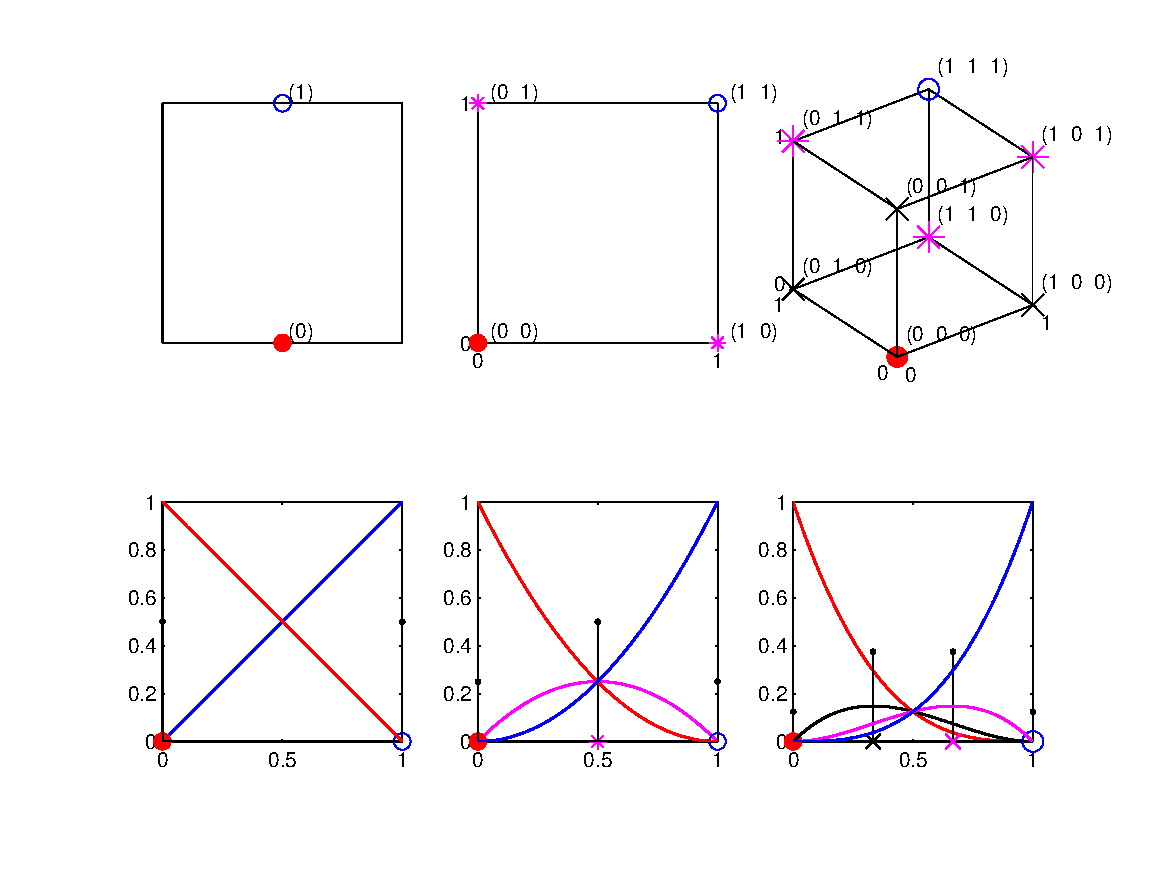
\includegraphics[width=4.5in]{figures/BernoulliSampleLkl}}
\end{figure}

\begin{figure}[ht]
\caption{{\small $100$ realisations of $C_{10}, C_{100}, C_{1000}$ based on samples of size $n$ $=$ $10$, $100$ and $1000$ drawn from the $\bernoulli(\theta^*=0.5)$ RV as per \hyperref[Mf:BernoulliMLEConsistency]{Labwork~\ref*{Mf:BernoulliMLEConsistency}}.  The MLE $\widehat{\theta}_n$ (cyan dot) and the log-likelihood function (magenta curve) for each of the $100$ replications of the experiment for each sample size $n$ are depicted.  The approximate normal-based $95\%$ confidence intervals with blue boundaries are based on the exact $\mathsf{se}_n=\sqrt{\theta^*(1-\theta^*)/n}=\sqrt{1/4}$, while those with red boundaries are based on the estimated $\widehat{\mathsf{se}_n}=\sqrt{\widehat{\theta}_n(1-\widehat{\theta}_n)/n}$.  The fraction of times the true parameter $\theta^*=0.5$ was engulfed by the exact and approximate confidence interval (empirical coverage) over the $100$ replications of the experiment for each of the three sample sizes are given by the numbers after {\tt Cvrg.=} and {\tt $\sim$=}, above each sub-plot, respectively.}\label{F:BernoulliMLEConsistency}}
\begin{center}
\makebox{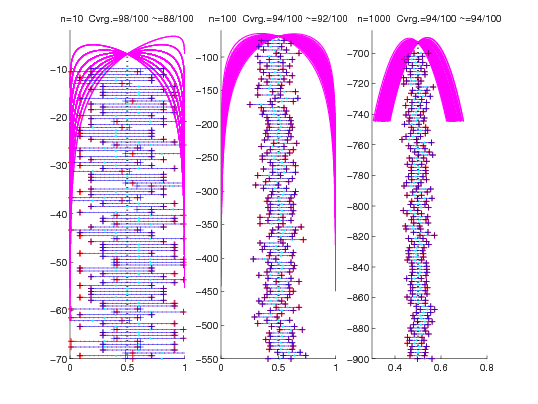
\includegraphics[width=4.50in]{figures/BernoulliMLEConsistency}}
\end{center}
\end{figure}  


%Let us look at some examples of estimation.
}



